Spočtěte určitý integrál
\begin{enumerate}

	\item $\int_0^1 (x^2+x+3) \dx$,

		\solution{
			$$\int_0^1 (x^2+x+3) \dx = \left[\frac{x^3}{3}+\frac{x^2}{2}+3x \right]_0^1 = \frac{1}{3} + \frac{1}{2} + 3 = \frac{23}{6}$$
		}

	\item $\int_0^\pi x \sin x \dx$,

		\solution{
			Pomocí integrace per partes určíme primitivní funkci 
			$$\int x \sin x \dx= -x \cos x - \int (-\cos x) \dx = -x \cos x + \int \cos x \dx =
			-x \cos x + \sin x +C$$
			$$\int_0^\pi x \sin x \dx = \left[-x \cos x + \sin x\right]_0^\pi = -\pi \cdot (-1)+0-(0 \cdot 1 +0) = \pi$$

			Geometrický význam vidíme na Obrázku~\ref{fig:xsinx}.
			\begin{figure}[H]
				\centering
				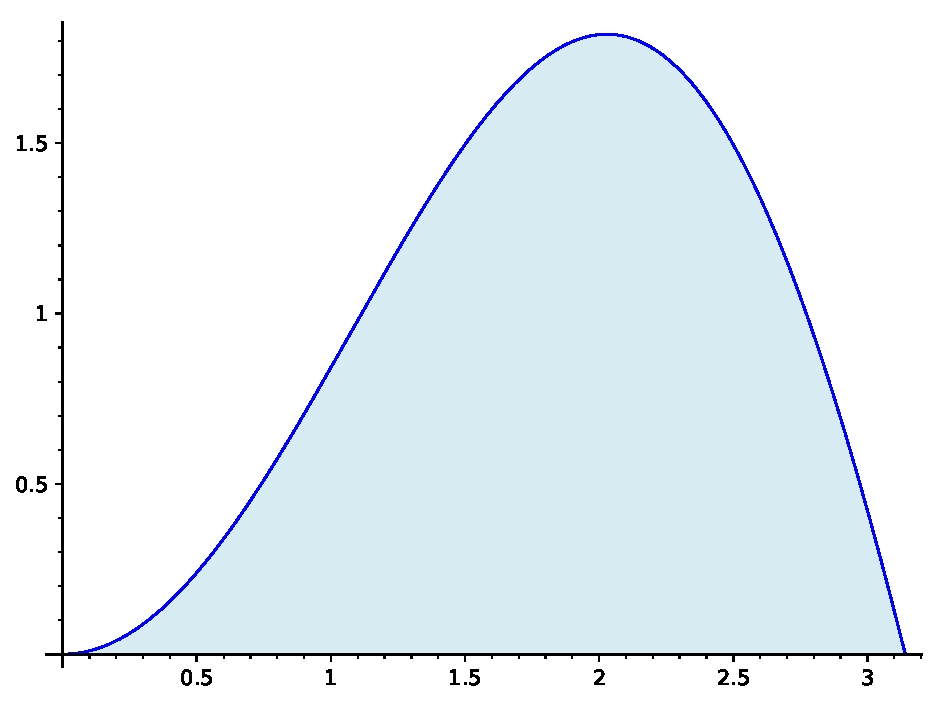
\includegraphics{cviceni_13/fig/xsinx.pdf}
				\caption{$\int_0^\pi x \sin x \dx = \pi$}
				\label{fig:xsinx}
			\end{figure}
		}

	\item $\int_1^2 x e^{x^2} \dx$,  

		\solution{
			Opět můžeme určit primitivní funkci a dosadit meze, ukážeme si ale počítání rovnou s mezemi (rozdíl se projeví kvůli substituci).

			Volíme substituci:
			\begin{align*}
				t &= x^2 \\
				\dt &= 2x \dx
			\end{align*}

			\begin{align*}
				\int_1^2 x e^{x^2} \dx &= \frac{1}{2} \int_1^2 e^{x^2} 2x \dx \\
				&= \frac{1}{2} \int_1^4 e^t \dt \\
				&= \frac{1}{2} [e^t]_1^4 \\
				&=  \frac{e^4 - e}{2}
			\end{align*}

			Obecně pokud volíme substituci:
			\begin{align*}
				t &= \varphi(x) \\
				\dx &= \varphi'(x) \dx
			\end{align*}
			pak máme:
			$$\int_{a}^{b} f(\varphi(x)) \varphi'(x) \dx = \int_{\varphi(a)}^{\varphi(b)} f(t) \dt$$
		}

	\item $\int_0^{\pi/4} \tan x \dx$.

		\solution{
			Volíme substituci:
			\begin{align*}
				t &= \cos(x) \\
				\dt &= -\sin(x) \dx
			\end{align*}

			\begin{align*}
				\int_0^{\pi/4} \tan x \dx &= -\int_0^{\pi/4} \frac{-\sin x}{\cos x} \dx \\
				&= - \int_{\cos(0)}^{\cos(\pi/4)} \frac{1}{t} \dt \\
				&= - \int_1^{1/\sqrt{2}} \frac{1}{t} \dt \\
				&= \int_{1/\sqrt{2}}^1 \frac{1}{t} \dt \\
				&= [\ln|t|]_{1/\sqrt{2}}^1 \\
				&= \ln(1) - \ln(1/\sqrt{2}) \\
				&= - \ln(1/\sqrt{2}) \\
				&= \ln(\sqrt{2}) \\
				&= \frac{\ln 2}{2} 
			\end{align*}
		}

\end{enumerate}

